\documentclass[10pt,foldmark,notumble]{leaflet}
\renewcommand*\foldmarkrule{.3mm}
\renewcommand*\foldmarklength{5mm}
\usepackage{float} %Bilder einbinden
\usepackage[utf8]{inputenc} %Umlaute
\usepackage{graphicx} %Graphiken
\usepackage{hyperref} %wg URL
\usepackage{amsmath}
\usepackage[T1]{fontenc}
\usepackage{textcomp}
\usepackage{mathptmx}
\usepackage{microtype}%Blocksatz
\usepackage[scaled=0.9]{helvet}

\usepackage[T1]{fontenc}
\newcommand{\changefont}[3]{
\fontfamily{#1} \fontseries{#2} \fontshape{#3} \selectfont} %http://www.math.tu-dresden.de/~rudl/latex/fonts.pdf


\makeatletter
\def\ptmTeX{T\kern-.1667em\lower.5ex\hbox{E}\kern-.075emX\@}
\DeclareRobustCommand{\ptmLaTeX}{L\kern-.3em
{\setbox0\hbox{T}%
%\vb@xt@ % :-)
\vbox to\ht0{\hbox{%
\csname S@\f@size\endcsname
\fontsize\sf@size\z@
\math@fontsfalse\selectfont
A}%
\vss}%
}%
\kern-.12em
\ptmTeX}
\makeatother
\let\TeX=\ptmTeX
\let\LaTeX=\ptmLaTeX
\usepackage{shortvrb}
\MakeShortVerb{\|}
\usepackage{url}
\usepackage[dvipsnames,usenames]{color}
\definecolor{LIGHTGRAY}{gray}{.9}
\newcommand\Lpack[1]{\textsf{#1}}
\newcommand\Lclass[1]{\textsf{#1}}
\newcommand\Lopt[1]{\texttt{#1}}
\newcommand\Lprog[1]{\textit{#1}}

\newcommand*\defaultmarker{\textsuperscript\textasteriskcentered}

%\CutLine*{1}% Dotted line without scissors
%\CutLine{6}% Dotted line with scissors
%\CutLine*{6}% 

%%%%%%%%%%%%%%%%%%%%%%%%%%%%%%%%%%%%%%%%%%%%%%%%%%%%%%%%%%%%%%%%%%%%%
\begin{document}

%\vspace*{20mm}
\section{Preisliste}
\begin{tabular}{p{35mm}lcr}%\hline\hline %
\\
\hline
\\
Geistheilung &   60/90 min. & 45/60,-€   \\
\\
\hline
\\
Bei Tieren   & 15 min. &  15,-€ \\
(Hausbesuch) & & \\
\\
\hline
\\
Klangmassage   & 30 min. &  20,-€ \\
\\
\hline
\\
Hot Stone Massage   & 30 min. & 25,-€   \\
\\
\hline 
\\
Atlantische Lichtheilung  & 60 min. &  45,-€ \\
\\
\hline
\\
Energetische  & 30 min. &  20,-€ \\
Rückenarbeit& &\\
\\
\hline
\\
Rückenmassage   & 30 min. & 20,-€ \\
(klassisch)& &\\
\\
\hline
\\
Ganzkörpermassage & 60 min. & 50,-€ \\
\\
\hline
\\
Beratungen & 60 min. & 45,-€ \\
\\
\hline
\\
%\multicolumn{2}{l}{kosmetische Fußpflege}\\
kosmetische Fußpflege & & 19,-€\\
(Hausbesuche) & & \\
\multicolumn{2}{l}{- keine Diabetiker }\\
\multicolumn{2}{l}{- keine Personen, die Blutverdünnungs-}\\
\multicolumn{2}{l}{~ medikamente einnehmen}\\
\\
\hline
\\
\multicolumn{3}{l}{Behandlungszeiten beinhalten Vor- und Nachgespräche.}\\
\\
\hline
\end{tabular} %\-




\newpage
%%%%%%%%%%%%%%%%%%%%%%%%%%%%%%%%%%%%%%%%%%%%%%%%%%%%%%%%%%%%%%%%%%%%%
%\vspace*{10mm} %{\bf}

\section{Massagetherapeutin}
Ausbildung 2004 in der Schweiz

\section{Mein Angebot für Sie:}

\begin{itemize}
\item {\bf klassische Ganzkörpermassage} \\
\item  {\bf Rücken oder Teilmassage} \\               
\item  {\bf Energetische Rückenarbeit}\\                
Eine sehr sanfte, langsame Massage bei der sehr viel Energie in Ihren ganzen Körper fließt. Eine wohlige Wärme erfüllt dabei ihren Körper und Sie fühlen sich leicht. Besonders geeignet bei Stress, depressiven Stimmungen, und "nicht zur Ruhe kommen."\\
\item  {\bf Klangmasse mit tibetischen Klangschalen}\\
Bringt Zell- und Körperflüssigkeiten in Fluss. Dadurch lösen sich Stauungen, Verhärtungen und Verspannungen.\\
\item  {\bf Hot Stone Massage/ heiße Steine}\\
Heiße Basaltsteine werden aufgelegt und damit massiert. Die Wirkung beruht auf einer umfassenden Aktivierung der Körpervorgänge, und es gibt fast keinen Aspekt im Organismus der von Ihrer Wirkung ausgeschlossen bleibt.\\
\begin{itemize}
\item Verbesserung der Durchblutung,
\item Verstärkung des Lymphflusses, 
\item Verbesserung des Gewebestoffwechsels,
\item Abtransport von Schlackenstoffen,
\item Lösen von Muskelverspannungen,
\item Einsetzbar bei Gelenkproblemen, Rückenschmerzen, Muskulatur,
\item Beruhigende Wirkung bei Stress,
\item Linderung von stressbedingten Spannungszuständen und deren Auswirkungen ( z.bsp. Kopfschmerzen, Schlaflosigkeit, Verdauungsprobleme), 
\item Stärkung des Immunsystems.
\end{itemize}
\end{itemize}
%
%%%%%%%%%%%%%%%%%%%%%%%%%%%%%%%%%%%%%%%%%%%%%%%%%%%%%%%%%%%%%%%%%%%%%
\newpage
\vspace*{15mm}
\centerline {\LARGE {\bf {Hier praktiziere ich}}}

\begin{figure}[h]
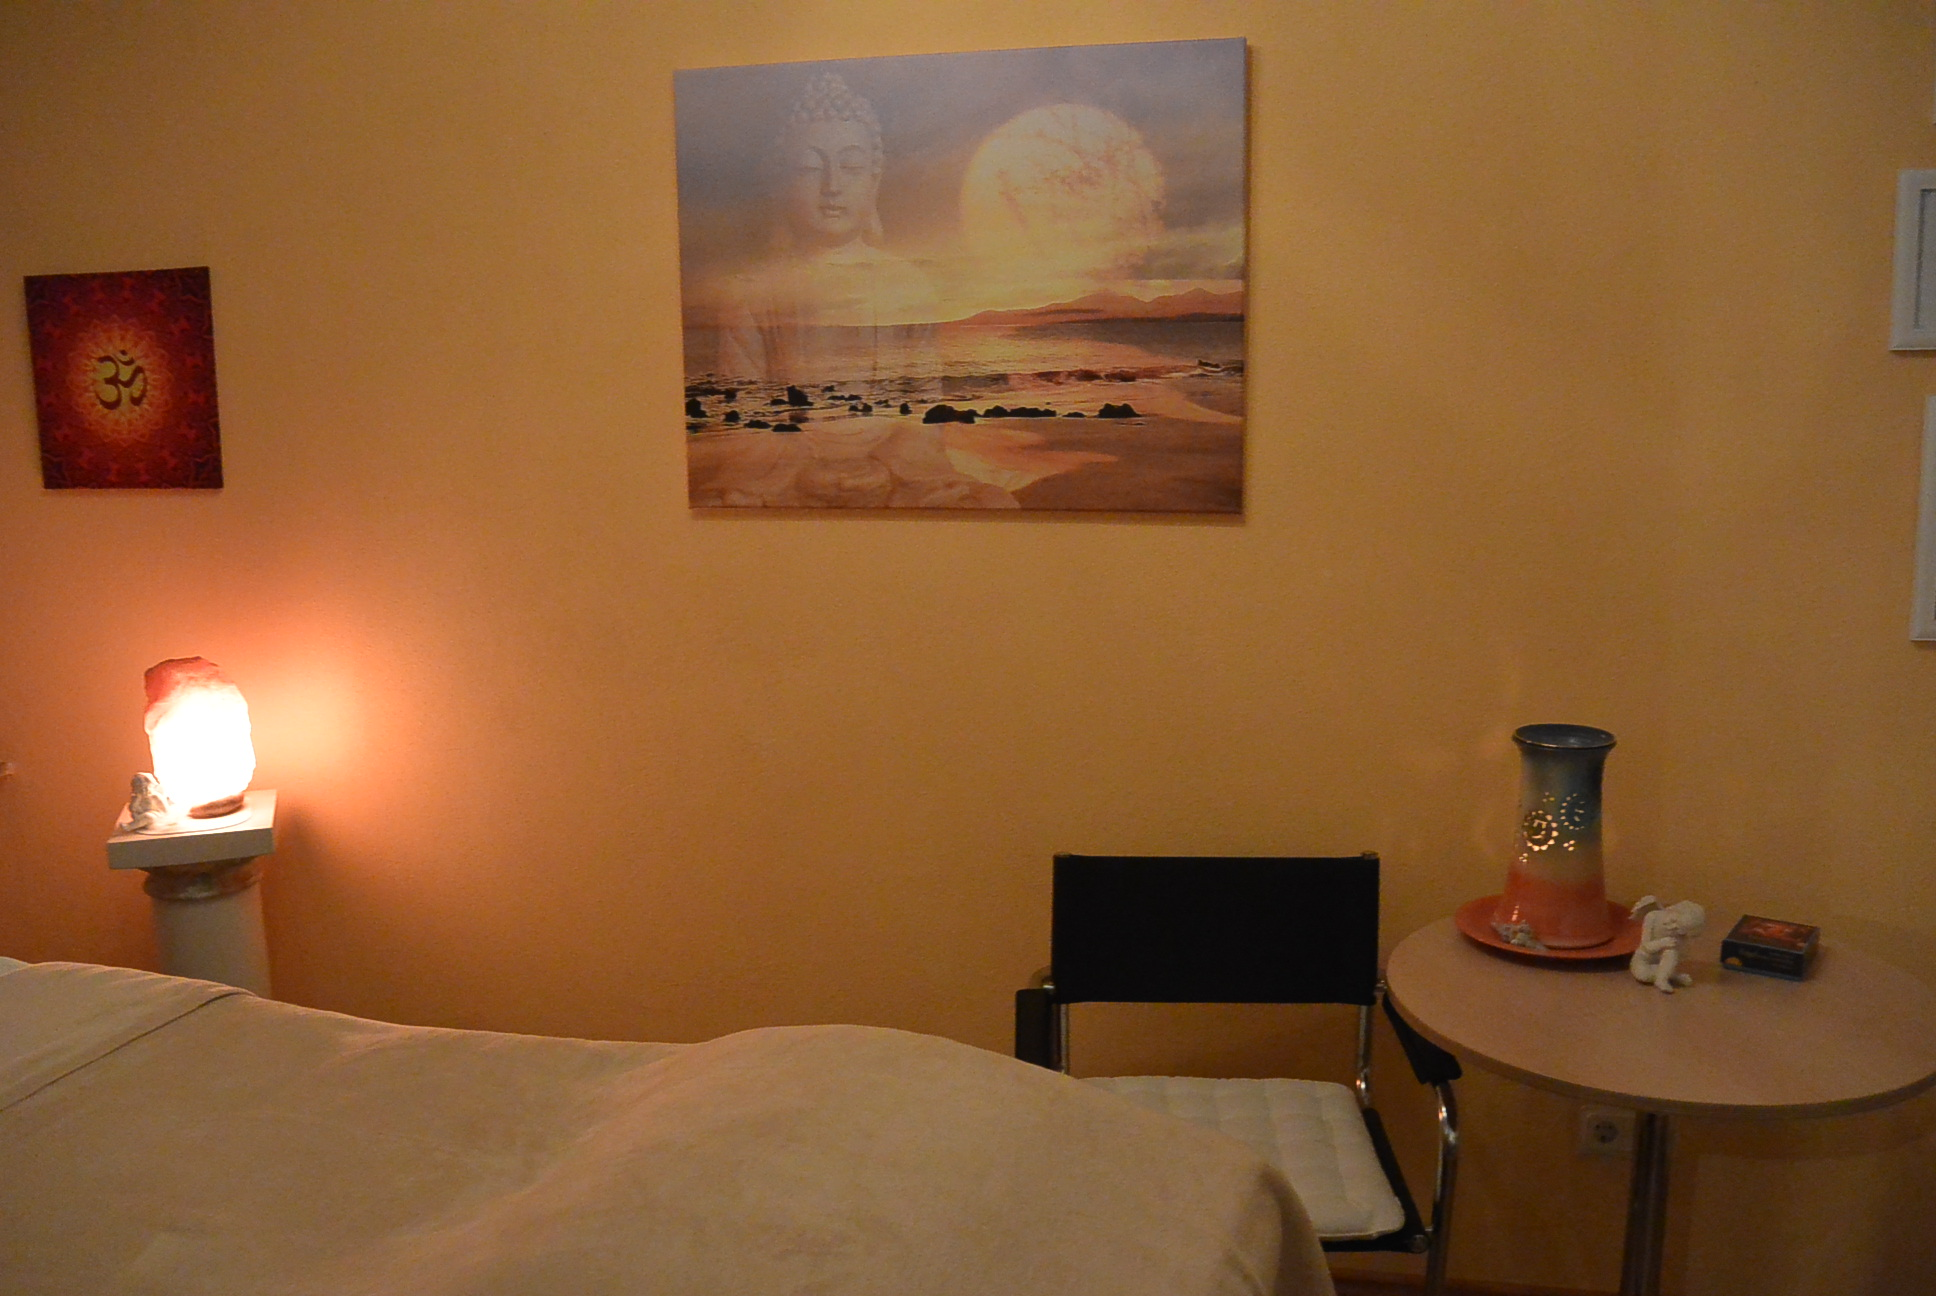
\includegraphics [scale=.12]{Raum_neu.jpg}
\end{figure}


\vspace*{7mm}
\begin{flushleft}
Saarwellingen\\
Dillinger Straße 15\\
Tel.: (0 68 38) 99 30 80\\
\href{mailto:gertrudschack@gmail.com}{gertrudschack@gmail.com} \\
\vspace{2mm}
\large{Termine nach Vereinbarung} %{\bf}\\
\end{flushleft}

%\section{ }
{\bf Meine Anwendungen dienen der Entspannung und \mbox{regen} die Selbstheilungskräfte an. Sie ersetzen nicht den Arzt oder den Heilpraktiker. }


%%%%%%%%%%%%%%%%%%%%%%%%%%%%%%%%%%%%%%%%%%%%%%%%%%%%%%%%%%%%%%%%%%%%%
\newpage
%\vspace*{15mm}

\centerline {\LARGE {\bf \it {Leben in Balance}}}

%\vspace*{32mm}
\begin{figure}[h] %[b]
\begin{center}
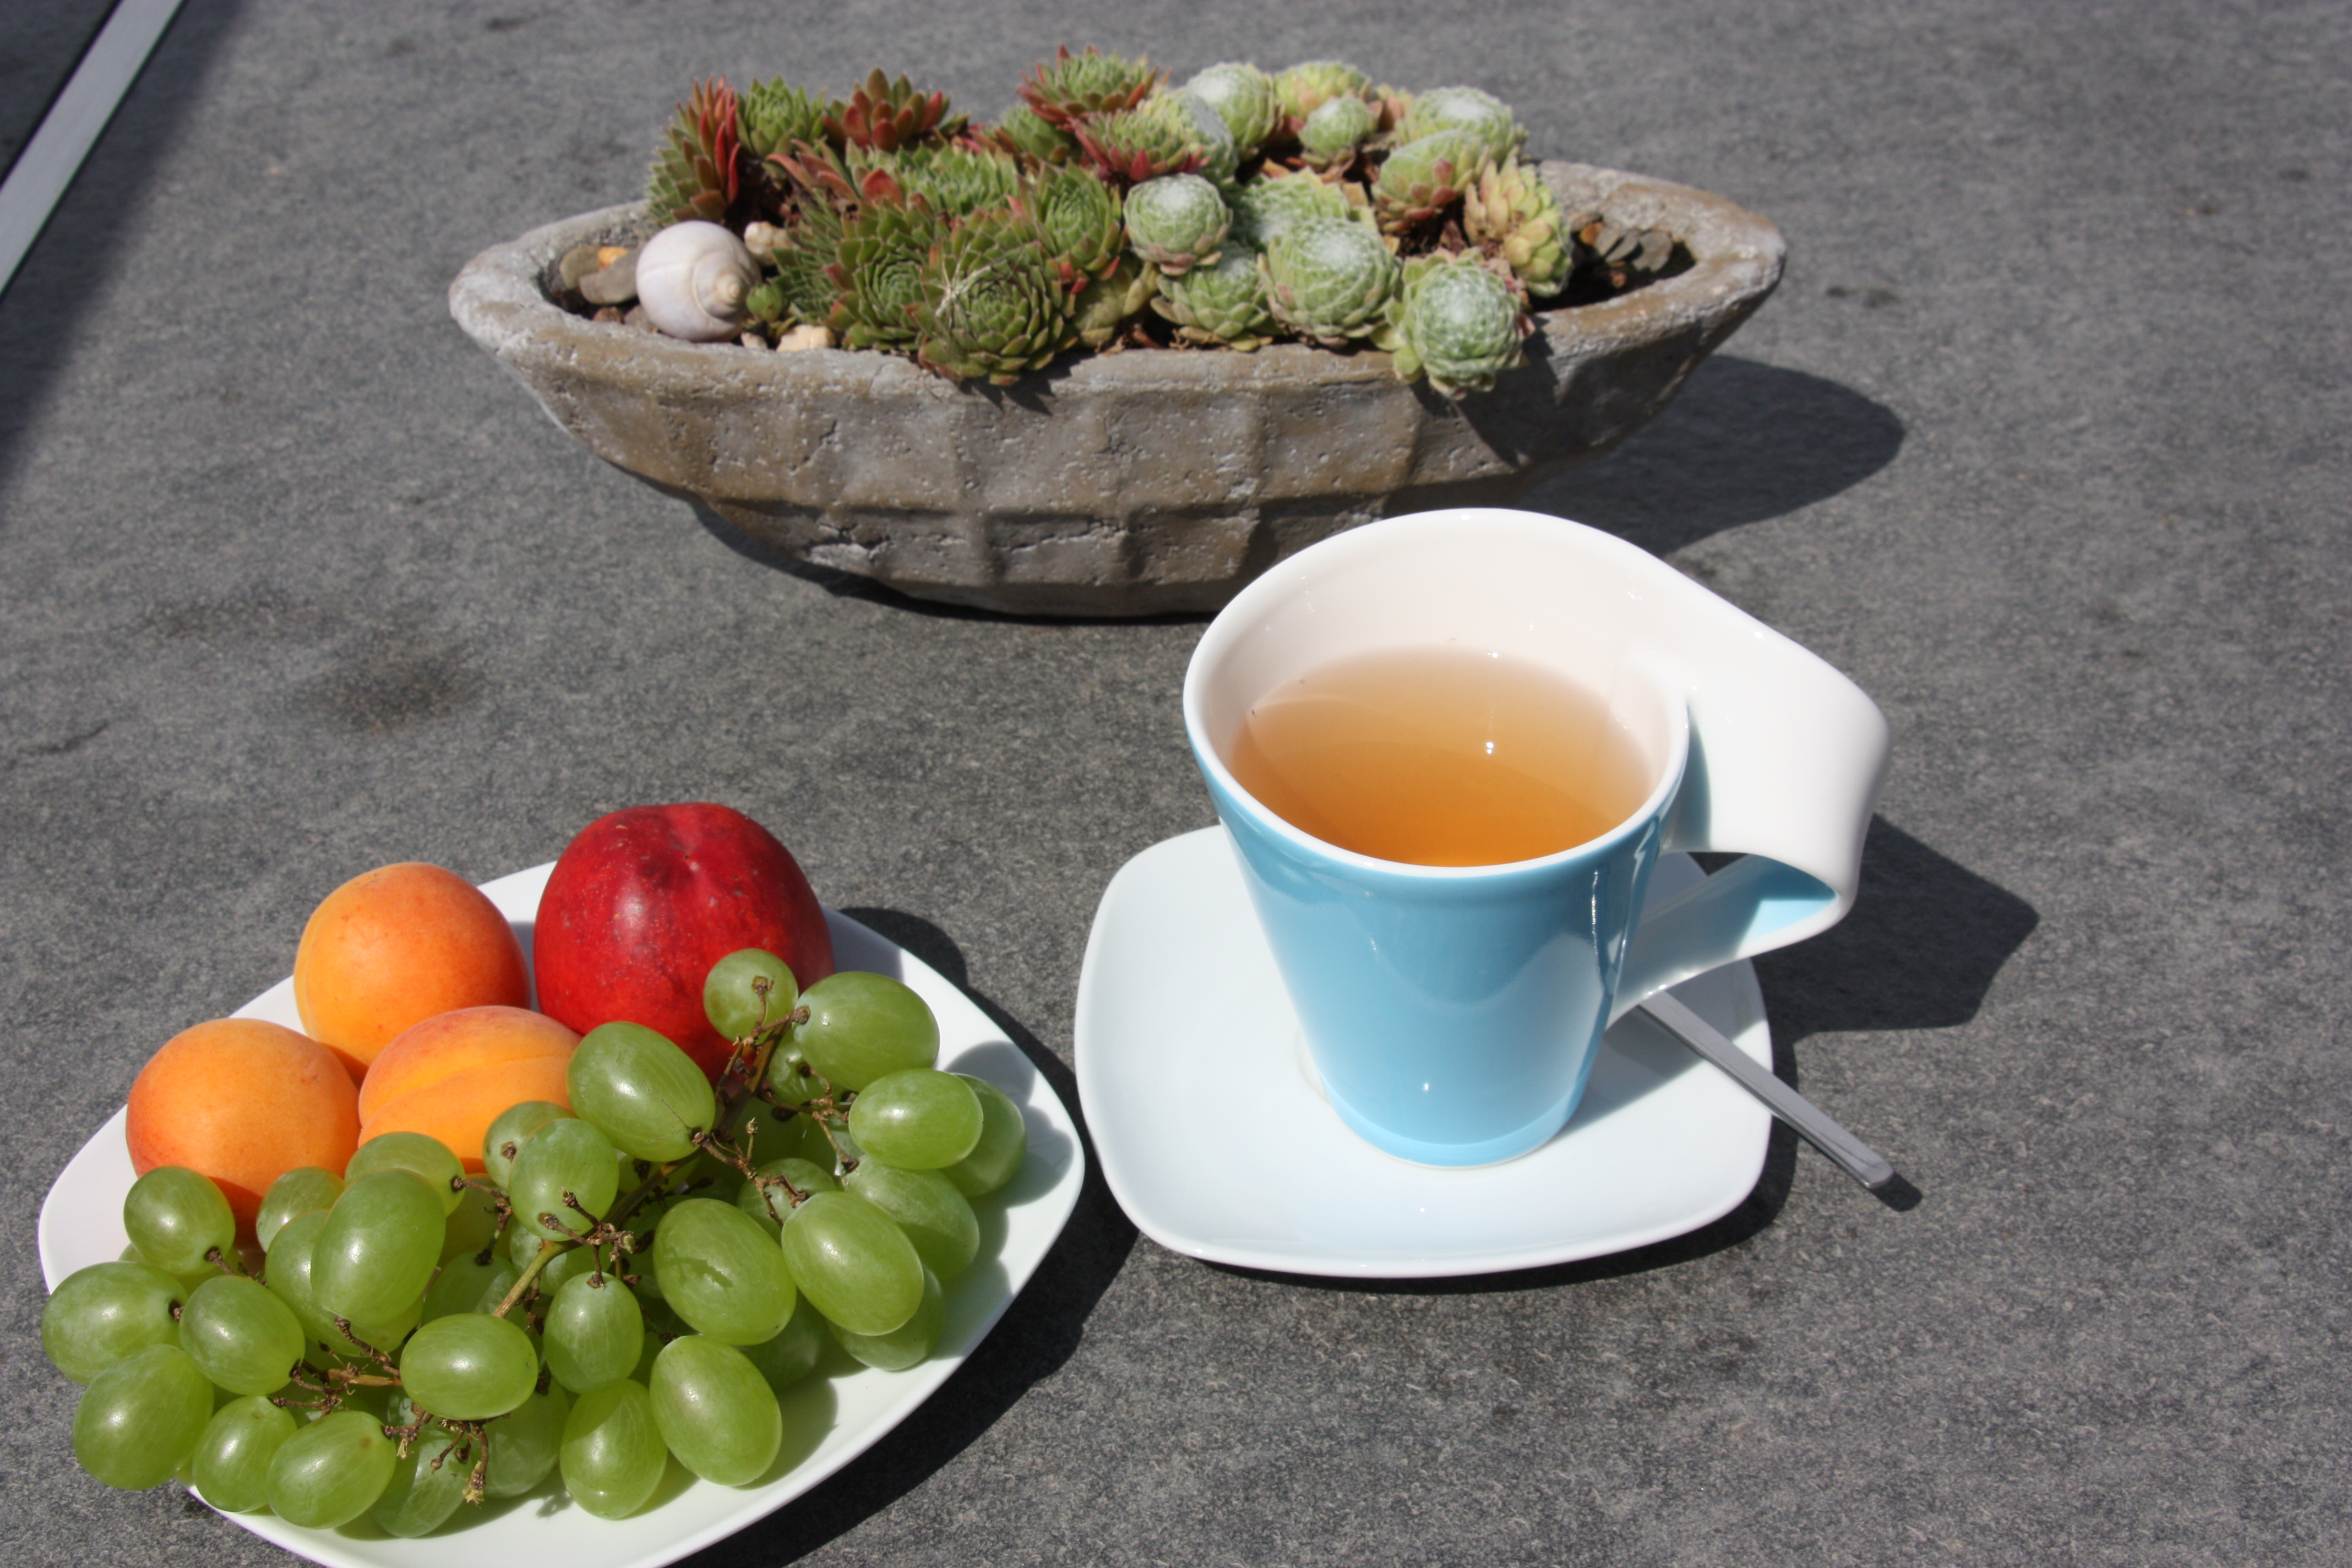
\includegraphics [scale=.055]{Bild_Fasten.JPG}
\end{center}
\end{figure}

\begin{center}
{\LARGE \bf {Gertrud Schack}}\\
\vspace*{5mm}
%\end{center}
%\begin{center}
\large {Atlantis Lichtheilung} \\ %\bf 
\vspace*{1mm}
\large {Massagetherapeutin} \\ 
\vspace*{1mm}
\large {Beraterin für Ernährung } \\ % 
\vspace*{1mm}
\large {Entschlackung \& Fasten} \\ 
\vspace*{1mm}
\large {Psychologische Beratung} \\ 
\vspace*{1mm}
\large {Med. Fußpflegerin} \\ 
%\vspace*{1mm}

\end{center}


%%%%%%%%%%%%%%%%%%%%%%%%%%%%%%%%%%%%%%%%%%%%%%%%%%%%%%%%%%%%%%%%%%%%%
\newpage
\section{Geistheilung durch Handauflegen}

Seit 1992 praktiziere ich Energiearbeit mit Reiki.\\ 
\\ 
2010 wurde ich in die höher und schnellerschwingende Atlantis Lichtheilung eingestimmt.\\
\\
Während der Behandlung wird durch meine Hände, die ich mit Abstand oder direkt, sanft auf Ihren Körper auflege, Energie zugeführt.\\
\\
Sie spüren wohltuend warme Hände, eventuell, einen \mbox{leichten} Energiefluss in Form von Kribbeln oder strömen. Sie entspannen tief. Ihre Selbstregulierungs- und Heilungskräfte werden sichtbar zum Beispiel in Kirlianfotografien.






%%%%%%%%%%%%%%%%%%%%%%%%%%%%%%%%%%%%%%%%%%%%%%%%%%%%%%%%%%%%%%%%%%%%%
\newpage


\section{Psychologische Beraterin seit 2007}
%{\bf Psychologische Beraterin seit 2007}\\

\vspace{2mm}

{\bf Ich bin gerne für Sie da}\\
\begin{itemize}
\item  für ein klärendes Gespräch,
\item  für tröstende Worte in einer schwierigen Lebenssituation,
\item  für Impulse zur Veränderung im privaten und beruflichen Beziehungen,
\item  für aufmerksames Zuhören,
\item  für Impulse zu einer gesunden Lebensgestaltung.
\end{itemize}

\vspace{2mm}

{\bf Beraterin für Ernährung, Gesundheit und Umwelt BEGU Frankfurt/Main 2007}\\

\vspace{2mm}

{\bf Ausbildung zur ganzheitlichen Fastenleiterin 1997}\\

\vspace{2mm}

{\bf Beraterin für Entschlackungskuren bei Peter \mbox{Jenschura} 1998}\\
\begin{itemize}
\item  Gespräche über Ihre Ernährung,
\item  Empfehlungen zur Ernährungsumstellung,
\item  einen Weg finden, für eine Ihnen entsprechende Ernährung,
\item  Begleitung bei Fastentagen,
\item  Beratung zur Entschlackung und Entsäuerung,
\item  Gespräche über gesundheitliche Themen.
\end{itemize}




%%%%%%%%%%%%%%%%%%%%%%%%%%%%%%%%%%%%%%%%%%%%%%%%%%%%%%%%%%%%%%%%%%%%%'
\end{document}